\documentclass{standalone}
\usepackage{tikz}
\usetikzlibrary{patterns, positioning}


\begin{document}
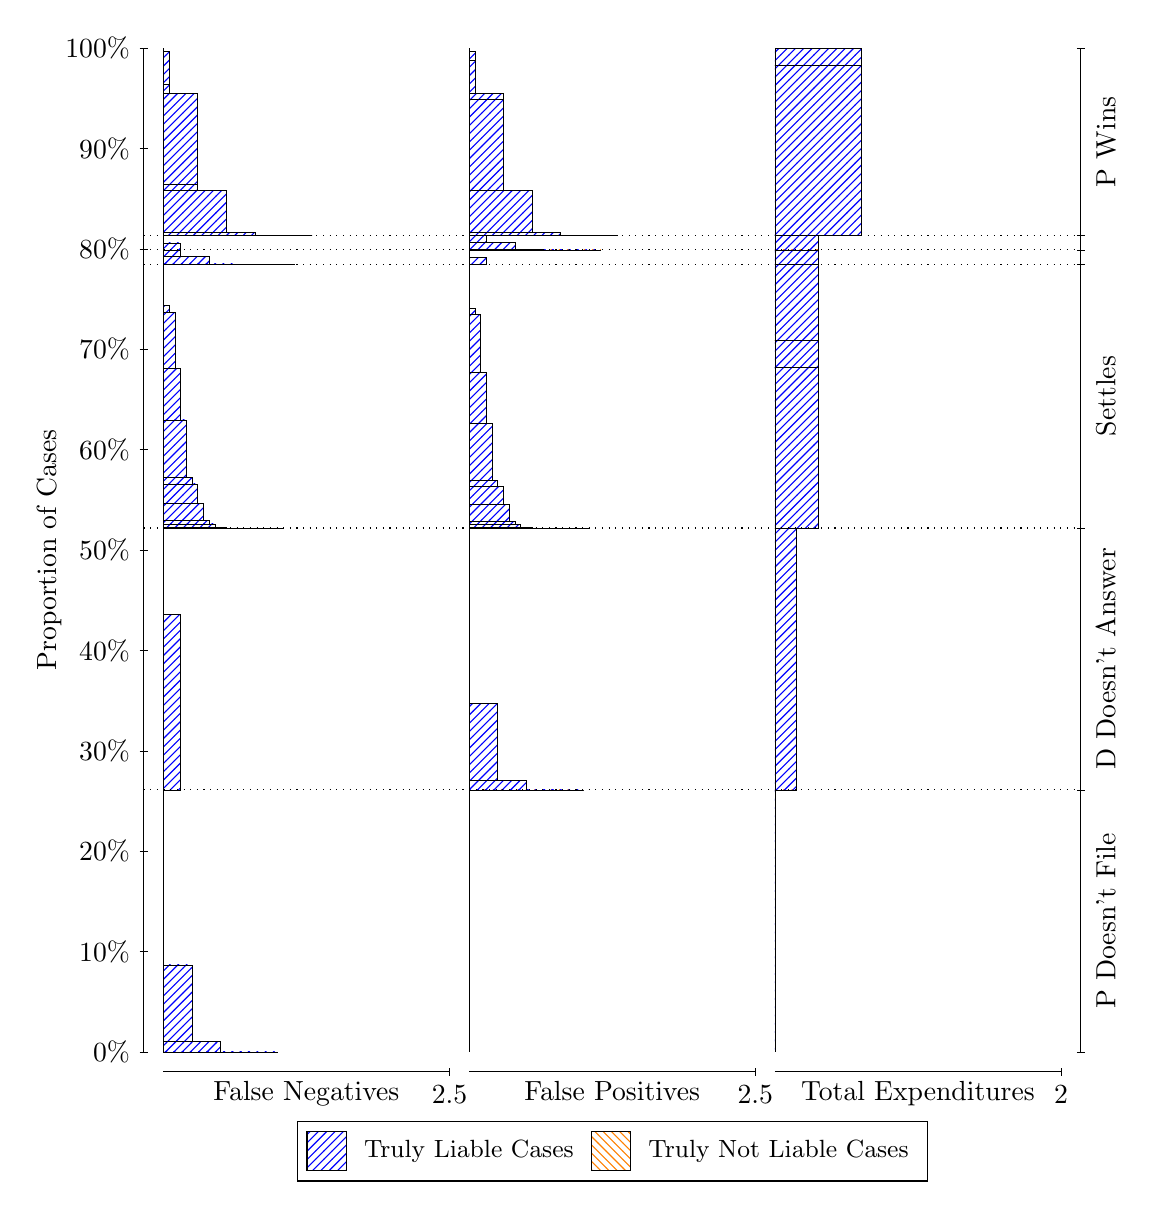
\begin{tikzpicture}
\draw[black, very thin] (1.5,1.75) -- (1.5,14.5);
\node[rotate=90, text=black, anchor=center] at (0.3, 8.125) {Proportion of Cases};
\draw[black, very thin] (1.45,1.75) -- (1.55,1.75);
\node[text=black, anchor=east] at (1.45, 1.75) {0\%};
\draw[black, very thin] (1.45,3.025) -- (1.55,3.025);
\node[text=black, anchor=east] at (1.45, 3.025) {10\%};
\draw[black, very thin] (1.45,4.3) -- (1.55,4.3);
\node[text=black, anchor=east] at (1.45, 4.3) {20\%};
\draw[black, very thin] (1.45,5.575) -- (1.55,5.575);
\node[text=black, anchor=east] at (1.45, 5.575) {30\%};
\draw[black, very thin] (1.45,6.85) -- (1.55,6.85);
\node[text=black, anchor=east] at (1.45, 6.85) {40\%};
\draw[black, very thin] (1.45,8.125) -- (1.55,8.125);
\node[text=black, anchor=east] at (1.45, 8.125) {50\%};
\draw[black, very thin] (1.45,9.4) -- (1.55,9.4);
\node[text=black, anchor=east] at (1.45, 9.4) {60\%};
\draw[black, very thin] (1.45,10.675) -- (1.55,10.675);
\node[text=black, anchor=east] at (1.45, 10.675) {70\%};
\draw[black, very thin] (1.45,11.95) -- (1.55,11.95);
\node[text=black, anchor=east] at (1.45, 11.95) {80\%};
\draw[black, very thin] (1.45,13.225) -- (1.55,13.225);
\node[text=black, anchor=east] at (1.45, 13.225) {90\%};
\draw[black, very thin] (1.45,14.5) -- (1.55,14.5);
\node[text=black, anchor=east] at (1.45, 14.5) {100\%};

\draw[black, very thin] (13.4,1.75) -- (13.4,14.5);
\draw[black, very thin] (13.35,1.75) -- (13.45,1.75);
\node[anchor=west] at (13.35, 1.75) {};
\draw[black, very thin] (13.35,5.0793) -- (13.45,5.0793);
\node[anchor=west] at (13.35, 5.0793) {};
\draw[black, very thin] (13.35,8.4039) -- (13.45,8.4039);
\node[anchor=west] at (13.35, 8.4039) {};
\draw[black, very thin] (13.35,11.756) -- (13.45,11.756);
\node[anchor=west] at (13.35, 11.756) {};
\draw[black, very thin] (13.35,11.937) -- (13.45,11.937);
\node[anchor=west] at (13.35, 11.937) {};
\draw[black, very thin] (13.35,12.119) -- (13.45,12.119);
\node[anchor=west] at (13.35, 12.119) {};
\draw[black, very thin] (13.35,14.5) -- (13.45,14.5);
\node[anchor=west] at (13.35, 14.5) {};

\draw[black, very thin, pattern color=blue, pattern=north east lines] (1.75,1.75) rectangle (3.2033,1.75);
\draw[black, very thin, pattern color=blue, pattern=north east lines] (1.75,1.75) rectangle (2.84,1.7511);
\draw[black, very thin, pattern color=blue, pattern=north east lines] (1.75,1.7511) rectangle (2.4767,1.8853);
\draw[black, very thin, pattern color=blue, pattern=north east lines] (1.75,1.8853) rectangle (2.1133,2.8548);
\draw[black, very thin, pattern color=orange, pattern=north west lines] (1.75,2.8548) rectangle (1.75,2.8548);
\draw[black, very thin, pattern color=blue, pattern=north east lines] (1.75,2.8548) rectangle (1.75,5.0793);
\draw[black, very thin, pattern color=blue, pattern=north east lines] (1.75,5.0793) rectangle (1.968,7.3056);
\draw[black, very thin, pattern color=orange, pattern=north west lines] (1.75,7.3056) rectangle (1.75,7.3056);
\draw[black, very thin, pattern color=blue, pattern=north east lines] (1.75,7.3056) rectangle (1.75,8.4039);
\draw[black, very thin, pattern color=blue, pattern=north east lines] (1.75,8.4039) rectangle (3.276,8.4039);
\draw[black, very thin, pattern color=blue, pattern=north east lines] (1.75,8.4039) rectangle (2.9853,8.4039);
\draw[black, very thin, pattern color=blue, pattern=north east lines] (1.75,8.4039) rectangle (2.9127,8.4039);
\draw[black, very thin, pattern color=blue, pattern=north east lines] (1.75,8.4039) rectangle (2.6947,8.404);
\draw[black, very thin, pattern color=blue, pattern=north east lines] (1.75,8.404) rectangle (2.622,8.4043);
\draw[black, very thin, pattern color=blue, pattern=north east lines] (1.75,8.4043) rectangle (2.5493,8.415);
\draw[black, very thin, pattern color=blue, pattern=north east lines] (1.75,8.415) rectangle (2.404,8.4565);
\draw[black, very thin, pattern color=blue, pattern=north east lines] (1.75,8.4565) rectangle (2.3313,8.5053);
\draw[black, very thin, pattern color=blue, pattern=north east lines] (1.75,8.5053) rectangle (2.2587,8.7182);
\draw[black, very thin, pattern color=blue, pattern=north east lines] (1.75,8.7182) rectangle (2.186,8.9654);
\draw[black, very thin, pattern color=blue, pattern=north east lines] (1.75,8.9654) rectangle (2.1133,9.0447);
\draw[black, very thin, pattern color=blue, pattern=north east lines] (1.75,9.0447) rectangle (2.0407,9.7769);
\draw[black, very thin, pattern color=blue, pattern=north east lines] (1.75,9.7769) rectangle (1.968,10.428);
\draw[black, very thin, pattern color=blue, pattern=north east lines] (1.75,10.428) rectangle (1.8953,11.146);
\draw[black, very thin, pattern color=blue, pattern=north east lines] (1.75,11.146) rectangle (1.8227,11.228);
\draw[black, very thin, pattern color=orange, pattern=north west lines] (1.75,11.228) rectangle (1.75,11.228);
\draw[black, very thin, pattern color=blue, pattern=north east lines] (1.75,11.228) rectangle (1.75,11.756);
\draw[black, very thin, pattern color=blue, pattern=north east lines] (1.75,11.756) rectangle (3.4213,11.756);
\draw[black, very thin, pattern color=blue, pattern=north east lines] (1.75,11.756) rectangle (3.058,11.756);
\draw[black, very thin, pattern color=blue, pattern=north east lines] (1.75,11.756) rectangle (2.6947,11.758);
\draw[black, very thin, pattern color=blue, pattern=north east lines] (1.75,11.758) rectangle (2.3313,11.849);
\draw[black, very thin, pattern color=blue, pattern=north east lines] (1.75,11.849) rectangle (1.968,11.937);
\draw[black, very thin, pattern color=orange, pattern=north west lines] (1.75,11.937) rectangle (1.75,11.937);
\draw[black, very thin, pattern color=blue, pattern=north east lines] (1.75,11.937) rectangle (1.968,12.025);
\draw[black, very thin, pattern color=orange, pattern=north west lines] (1.75,12.025) rectangle (1.75,12.025);
\draw[black, very thin, pattern color=blue, pattern=north east lines] (1.75,12.025) rectangle (1.75,12.119);
\draw[black, very thin, pattern color=blue, pattern=north east lines] (1.75,12.119) rectangle (3.6393,12.119);
\draw[black, very thin, pattern color=blue, pattern=north east lines] (1.75,12.119) rectangle (3.276,12.119);
\draw[black, very thin, pattern color=blue, pattern=north east lines] (1.75,12.119) rectangle (2.9127,12.16);
\draw[black, very thin, pattern color=blue, pattern=north east lines] (1.75,12.16) rectangle (2.5493,12.695);
\draw[black, very thin, pattern color=blue, pattern=north east lines] (1.75,12.695) rectangle (2.186,12.771);
\draw[black, very thin, pattern color=blue, pattern=north east lines] (1.75,12.771) rectangle (2.186,13.924);
\draw[black, very thin, pattern color=blue, pattern=north east lines] (1.75,13.924) rectangle (1.8227,14.035);
\draw[black, very thin, pattern color=blue, pattern=north east lines] (1.75,14.035) rectangle (1.8227,14.459);
\draw[black, very thin, pattern color=orange, pattern=north west lines] (1.75,14.459) rectangle (1.75,14.459);
\draw[black, very thin, pattern color=blue, pattern=north east lines] (1.75,14.459) rectangle (1.75,14.5);
\draw[black, very thin, pattern color=orange, pattern=north west lines] (5.6333,1.75) rectangle (5.6333,1.75);
\draw[black, very thin, pattern color=blue, pattern=north east lines] (5.6333,1.75) rectangle (5.6333,5.0793);
\draw[black, very thin, pattern color=orange, pattern=north west lines] (5.6333,5.0793) rectangle (7.0867,5.0793);
\draw[black, very thin, pattern color=blue, pattern=north east lines] (5.6333,5.0793) rectangle (7.0867,5.0793);
\draw[black, very thin, pattern color=blue, pattern=north east lines] (5.6333,5.0793) rectangle (6.7233,5.0798);
\draw[black, very thin, pattern color=blue, pattern=north east lines] (5.6333,5.0798) rectangle (6.36,5.2016);
\draw[black, very thin, pattern color=blue, pattern=north east lines] (5.6333,5.2016) rectangle (5.9967,6.1776);
\draw[black, very thin, pattern color=blue, pattern=north east lines] (5.6333,6.1776) rectangle (5.6333,8.4039);
\draw[black, very thin, pattern color=orange, pattern=north west lines] (5.6333,8.4039) rectangle (7.1593,8.4039);
\draw[black, very thin, pattern color=blue, pattern=north east lines] (5.6333,8.4039) rectangle (7.1593,8.4039);
\draw[black, very thin, pattern color=orange, pattern=north west lines] (5.6333,8.4039) rectangle (6.8687,8.4039);
\draw[black, very thin, pattern color=blue, pattern=north east lines] (5.6333,8.4039) rectangle (6.8687,8.4039);
\draw[black, very thin, pattern color=blue, pattern=north east lines] (5.6333,8.4039) rectangle (6.796,8.4039);
\draw[black, very thin, pattern color=orange, pattern=north west lines] (5.6333,8.4039) rectangle (6.578,8.4039);
\draw[black, very thin, pattern color=blue, pattern=north east lines] (5.6333,8.4039) rectangle (6.578,8.4039);
\draw[black, very thin, pattern color=blue, pattern=north east lines] (5.6333,8.4039) rectangle (6.5053,8.4043);
\draw[black, very thin, pattern color=blue, pattern=north east lines] (5.6333,8.4043) rectangle (6.4327,8.4139);
\draw[black, very thin, pattern color=orange, pattern=north west lines] (5.6333,8.4139) rectangle (6.2873,8.4139);
\draw[black, very thin, pattern color=blue, pattern=north east lines] (5.6333,8.4139) rectangle (6.2873,8.4543);
\draw[black, very thin, pattern color=blue, pattern=north east lines] (5.6333,8.4543) rectangle (6.2147,8.4927);
\draw[black, very thin, pattern color=blue, pattern=north east lines] (5.6333,8.4927) rectangle (6.142,8.7053);
\draw[black, very thin, pattern color=blue, pattern=north east lines] (5.6333,8.7053) rectangle (6.0693,8.9313);
\draw[black, very thin, pattern color=orange, pattern=north west lines] (5.6333,8.9313) rectangle (5.9967,8.9313);
\draw[black, very thin, pattern color=blue, pattern=north east lines] (5.6333,8.9313) rectangle (5.9967,9.0137);
\draw[black, very thin, pattern color=blue, pattern=north east lines] (5.6333,9.0137) rectangle (5.924,9.7319);
\draw[black, very thin, pattern color=blue, pattern=north east lines] (5.6333,9.7319) rectangle (5.8513,10.383);
\draw[black, very thin, pattern color=blue, pattern=north east lines] (5.6333,10.383) rectangle (5.7787,11.115);
\draw[black, very thin, pattern color=blue, pattern=north east lines] (5.6333,11.115) rectangle (5.706,11.194);
\draw[black, very thin, pattern color=blue, pattern=north east lines] (5.6333,11.194) rectangle (5.6333,11.756);
\draw[black, very thin, pattern color=orange, pattern=north west lines] (5.6333,11.756) rectangle (5.8513,11.756);
\draw[black, very thin, pattern color=blue, pattern=north east lines] (5.6333,11.756) rectangle (5.8513,11.843);
\draw[black, very thin, pattern color=blue, pattern=north east lines] (5.6333,11.843) rectangle (5.6333,11.937);
\draw[black, very thin, pattern color=orange, pattern=north west lines] (5.6333,11.937) rectangle (7.3047,11.937);
\draw[black, very thin, pattern color=blue, pattern=north east lines] (5.6333,11.937) rectangle (7.3047,11.937);
\draw[black, very thin, pattern color=blue, pattern=north east lines] (5.6333,11.937) rectangle (6.9413,11.937);
\draw[black, very thin, pattern color=blue, pattern=north east lines] (5.6333,11.937) rectangle (6.578,11.939);
\draw[black, very thin, pattern color=blue, pattern=north east lines] (5.6333,11.939) rectangle (6.2147,12.031);
\draw[black, very thin, pattern color=blue, pattern=north east lines] (5.6333,12.031) rectangle (5.8513,12.119);
\draw[black, very thin, pattern color=orange, pattern=north west lines] (5.6333,12.119) rectangle (7.5227,12.119);
\draw[black, very thin, pattern color=blue, pattern=north east lines] (5.6333,12.119) rectangle (7.5227,12.119);
\draw[black, very thin, pattern color=orange, pattern=north west lines] (5.6333,12.119) rectangle (7.1593,12.119);
\draw[black, very thin, pattern color=blue, pattern=north east lines] (5.6333,12.119) rectangle (7.1593,12.119);
\draw[black, very thin, pattern color=orange, pattern=north west lines] (5.6333,12.119) rectangle (6.796,12.119);
\draw[black, very thin, pattern color=blue, pattern=north east lines] (5.6333,12.119) rectangle (6.796,12.16);
\draw[black, very thin, pattern color=orange, pattern=north west lines] (5.6333,12.16) rectangle (6.4327,12.16);
\draw[black, very thin, pattern color=blue, pattern=north east lines] (5.6333,12.16) rectangle (6.4327,12.695);
\draw[black, very thin, pattern color=blue, pattern=north east lines] (5.6333,12.695) rectangle (6.0693,13.848);
\draw[black, very thin, pattern color=orange, pattern=north west lines] (5.6333,13.848) rectangle (6.0693,13.848);
\draw[black, very thin, pattern color=blue, pattern=north east lines] (5.6333,13.848) rectangle (6.0693,13.924);
\draw[black, very thin, pattern color=blue, pattern=north east lines] (5.6333,13.924) rectangle (5.706,14.345);
\draw[black, very thin, pattern color=blue, pattern=north east lines] (5.6333,14.345) rectangle (5.706,14.459);
\draw[black, very thin, pattern color=blue, pattern=north east lines] (5.6333,14.459) rectangle (5.6333,14.5);
\draw[black, very thin, pattern color=orange, pattern=north west lines] (9.5167,1.75) rectangle (9.5167,1.75);
\draw[black, very thin, pattern color=blue, pattern=north east lines] (9.5167,1.75) rectangle (9.5167,5.0793);
\draw[black, very thin, pattern color=orange, pattern=north west lines] (9.5167,5.0793) rectangle (9.7892,5.0793);
\draw[black, very thin, pattern color=blue, pattern=north east lines] (9.5167,5.0793) rectangle (9.7892,8.4039);
\draw[black, very thin, pattern color=orange, pattern=north west lines] (9.5167,8.4039) rectangle (10.062,8.4039);
\draw[black, very thin, pattern color=blue, pattern=north east lines] (9.5167,8.4039) rectangle (10.062,10.444);
\draw[black, very thin, pattern color=orange, pattern=north west lines] (9.5167,10.444) rectangle (10.062,10.444);
\draw[black, very thin, pattern color=blue, pattern=north east lines] (9.5167,10.444) rectangle (10.062,10.784);
\draw[black, very thin, pattern color=orange, pattern=north west lines] (9.5167,10.784) rectangle (10.062,10.784);
\draw[black, very thin, pattern color=blue, pattern=north east lines] (9.5167,10.784) rectangle (10.062,11.756);
\draw[black, very thin, pattern color=orange, pattern=north west lines] (9.5167,11.756) rectangle (10.062,11.756);
\draw[black, very thin, pattern color=blue, pattern=north east lines] (9.5167,11.756) rectangle (10.062,11.937);
\draw[black, very thin, pattern color=orange, pattern=north west lines] (9.5167,11.937) rectangle (10.062,11.937);
\draw[black, very thin, pattern color=blue, pattern=north east lines] (9.5167,11.937) rectangle (10.062,12.119);
\draw[black, very thin, pattern color=orange, pattern=north west lines] (9.5167,12.119) rectangle (10.607,12.119);
\draw[black, very thin, pattern color=blue, pattern=north east lines] (9.5167,12.119) rectangle (10.607,14.283);
\draw[black, very thin, pattern color=orange, pattern=north west lines] (9.5167,14.283) rectangle (10.607,14.283);
\draw[black, very thin, pattern color=blue, pattern=north east lines] (9.5167,14.283) rectangle (10.607,14.5);
\draw[black, dotted] (1.5,5.0793) -- (13.4,5.0793);
\draw[black, dotted] (1.5,8.4039) -- (13.4,8.4039);
\draw[black, dotted] (1.5,11.756) -- (13.4,11.756);
\draw[black, dotted] (1.5,11.937) -- (13.4,11.937);
\draw[black, dotted] (1.5,12.119) -- (13.4,12.119);
\draw[black, very thin] (1.75,1.5) -- (5.3833,1.5);
\node[text=black, anchor=north] at (3.5667, 1.5) {False Negatives};
\draw[black, very thin] (5.3833,1.45) -- (5.3833,1.55);
\node[text=black, anchor=north] at (5.3833, 1.45) {2.5};

\draw[black, very thin] (5.6333,1.5) -- (9.2667,1.5);
\node[text=black, anchor=north] at (7.45, 1.5) {False Positives};
\draw[black, very thin] (9.2667,1.45) -- (9.2667,1.55);
\node[text=black, anchor=north] at (9.2667, 1.45) {2.5};

\draw[black, very thin] (9.5167,1.5) -- (13.15,1.5);
\node[text=black, anchor=north] at (11.333, 1.5) {Total Expenditures};
\draw[black, very thin] (13.15,1.45) -- (13.15,1.55);
\node[text=black, anchor=north] at (13.15, 1.45) {2};

\node[text=black, centered, rotate=90] at (13.72, 3.4146) {P Doesn't File};
\node[text=black, centered, rotate=90] at (13.72, 6.7416) {D Doesn't Answer};
\node[text=black, centered, rotate=90] at (13.72, 10.08) {Settles};


\node[text=black, centered, rotate=90] at (13.72, 13.309) {P Wins};

\draw (7.449999999999999,1.5) node[draw=none] (baseCoordinate) {};
\begin{scope}[align=center]
        \matrix[scale=0.5, draw=black, below=0.5cm of baseCoordinate, nodes={draw}, column sep=0.1cm]{
            \node[rectangle, draw, minimum width=0.5cm, minimum height=0.5cm, pattern color=blue, pattern=north east lines] {}; &
            \node[draw=none, font=\small, text=black] (B) {Truly Liable Cases}; &
            \node[rectangle, draw, minimum width=0.5cm, minimum height=0.5cm, pattern color=orange, pattern=north west lines] {}; &
            \node[draw=none, font=\small, text=black] (B) {Truly Not Liable Cases}; \\
            };
\end{scope}

\end{tikzpicture}
\end{document}